%
% File acl2014.tex
%
% Contact: giovanni.colavizza@epfl.ch
%%
%% Based on the style files for ACL-2013, which were, in turn,
%% Based on the style files for ACL-2012, which were, in turn,
%% based on the style files for ACL-2011, which were, in turn, 
%% based on the style files for ACL-2010, which were, in turn, 
%% based on the style files for ACL-IJCNLP-2009, which were, in turn,
%% based on the style files for EACL-2009 and IJCNLP-2008...

%% Based on the style files for EACL 2006 by 
%%e.agirre@ehu.es or Sergi.Balari@uab.es
%% and that of ACL 08 by Joakim Nivre and Noah Smith

\documentclass[11pt]{article}
\usepackage{acl2014}
\usepackage{times}
\usepackage{url}
\usepackage{latexsym}
\usepackage{float}
\usepackage{graphicx}

%\setlength\titlebox{5cm}

% You can expand the titlebox if you need extra space
% to show all the authors. Please do not make the titlebox
% smaller than 5cm (the original size); we will check this
% in the camera-ready version and ask you to change it back.


\title{Words and politics: how well does \textit{r/politics} mirror the reality}

\author{Arnaud Hennig \\
  {\tt arnaud.hennig@epfl.ch} \\\And
    \\
  {\tt  } \\\\
  \textbf{Nourchene Ben Romdhane} \\
  {\tt nourchene.benromdhane@epfl.ch} \\\And
Arthur Vernet \\
{\tt arthur.vernet@epfl.ch} \\}

\date{\today}

\begin{document}
\maketitle
\begin{abstract}
Focusing on a time-span covering the months of June 2016 to November 2016, i.e. the 6 months preceding the American election of 2016, this project aims at discovering the underlying patterns that make comments being deemed good by other users and understand how they correlate with actual events. It also aims at understanding the population of the subreddit \textit{r/politics} by analyzing its political spectrum and see how closely it relates to the outcome of the 2016 American election.
\end{abstract}

\section{Introduction}
The 2016 United States presidential American election is one of the most talked about event of these last few years, as it was the stage of one of the biggest political upsets ever seen in the United States of America. Beyond that, the election also came with its share of scandals.
This period of time appeared as a good opportunity to analyze how controversial events influence people's behaviour online, and how people's takes on the involved politicians fluctuates. In order to perform such an analysis, data from a well-known social network called Reddit was retrieved. Reddit, being the 5th most visited website in the USA and having more than half of its users originating from the USA\footnote{https://www.alexa.com/siteinfo/reddit.com}, seemed like the perfect place to conduct this experiment. \\
This study focuses on a specific community of Reddit, namely the users of the subreddit \textit{r/politics}. Subreddits are categories of the website focusing on specific topic, in this case \textit{r/politics} is a hub for everyone willing to read or discuss about the political landscape of the United States of America. It is obviously a highly political part of the website, where opinions diverge a lot, thus likely creating controversy. It is also one of the biggest subreddit, with more than 4 millions subscribers\footnote{https://www.reddit.com/r/politics/}. \\
Through the analysis of the comments posted on this website during the 6 months preceding the 2016 United States presidential American election, this project aims to understand what words or topics generated the most controversy or approval in this particular period, and how well the community of \textit{r/politics} is representative of the rest of the USA by trying to draw an estimation of the outcome of the election and comparing it with the reality. 

\section{Data collection}
Using Spark, the history of comments posted on \textit{r/politics} between June 2016 and November 2016 was retrieved from a massive dataset stored on the cluster dedicated for the class CS-401 Applied Data Analysis, consisting of the entirety of the comments posted on Reddit between 2007 and 2017. Figure \ref{time-distribution} showcases how the number of comments posted is correlated with important political events as high peaks match days where nationally televised debates took place as well as election day. 
Unfortunately, this dataset being still too large to be dealt with locally efficiently as it remained about 1.5Go big and contained more than 10 millions comments, a decision was taken to split it into two smaller datasets. Indeed, as the conducted analysis relied largely on natural language processing (NLP), it was unfeasible to process such large data. \\
As Reddit users are allowed to associate themselves with \textit{flairs} (understand tag) unique to each subreddit, and knowing that the \textit{flairs} of \textit{r/politics} contained the 50 states of the USA, a first dataset was generated keeping only comments whose author had one of these 50 specific flairs. The reason why this choice was made will become apparent later on. However, this newly generated dataset contains about 215'000 comments which makes it significantly smaller and processible. Note that, as Figure \ref{flair-distribution} proves it, certain states are underrepresented and may impact later on computations. \\
A second dataset was generated keeping comments whose score was bigger than a certain threshold and those whose score was smaller than a certain threshold. This way, the dataset mainly contains comments that generated high controversy and approval. It was also completed by sampling at random comments inbetween these two thresholds in order to have a dataset that remains representative of the overall population of \textit{r/politics}. This dataset also contains about 210'000 comments.

\begin{figure}
\centering
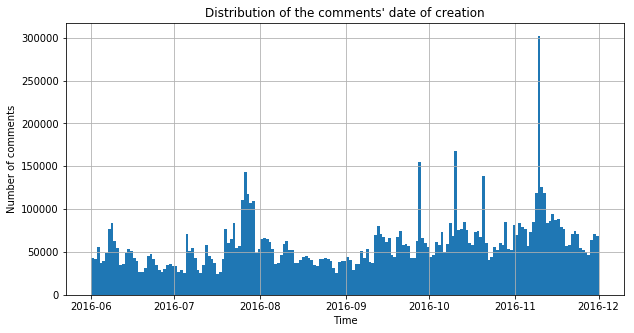
\includegraphics[scale=0.35]{Images/time-distribution.jpg}
\caption{Distribution of the number of comments across time for the original dataset.}
\label{time-distribution}
\end{figure}

\begin{figure}
\centering
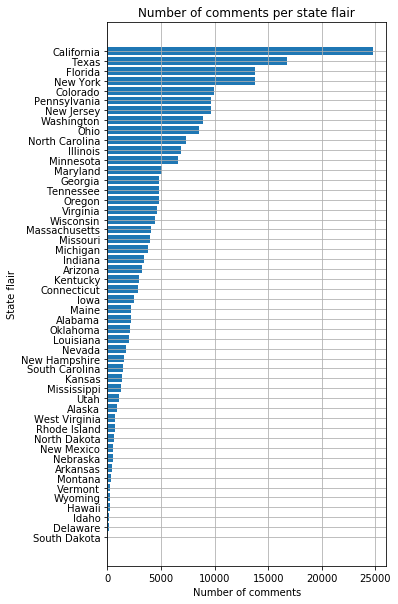
\includegraphics[scale=0.35]{Images/flair-distribution.jpg}
\caption{Distribution of the number of comments per state flair.}
\label{flair-distribution}
\end{figure}

\section{Dataset description}
The datasets consist of several different features listed below:
\begin{itemize}
    \item \textbf{author}: The username of the author of the comment.
    \item \textbf{author\_flair\_text}: The flair of the user.
    \item \textbf{body}: The content of the comment.
    \item \textbf{created\_utc}: The date at which the comment was originally posted.
    \item \textbf{score}: The number of upvotes minus the number of downvotes the comment received.
\end{itemize}
Additional features were then added using NLP over the body of the comments. First off, named entities mentioned in the comment (such as Hillary Clinton and Donald Trump) were isolated. Then the overall sentiment of the comment was computed using the NLTK sentiment package\footnote{https://www.nltk.org/api/nltk.sentiment.html} as its \textit{Vader} module is particularly useful, since it uses an already trained sentiment intensity analyzer. From this sentiment analysis, we labeled the comments as containing a positive, negative or neutral opinion. Finally, the word distribution was computed, by removing numeric values and \textit{stop-words} (common words such as the, a, he, has, was or to). The rest is then changed to lowercase and a lemmatizer was used to have a meaningful distribution. The added features are hence : 
\begin{itemize}
    \item \textbf{entity}: Named entities extracted from the comment's body.
    \item \textbf{sentiment}: 4 numeric values corresponding to a sentiment analysis ordered as such : compound, neg, neu, pos separated by a comma.
    \item \textbf{wordcount}: Dictionnary containing words frequencies.
    \item \textbf{label}: Classifying the comment as either Negative, Neutral or Positive.
\end{itemize}


\section{Methods}
At this point, the datasets contain all the necessary features to perform further analysis once a few methods are applied on them.
\subsection{Flairs}
Certain users have flairs of states, which most likely associate them with this particular state one way or another. For this part, we hence use the first generated data set which contains the comments with the author flair set to a US State. By assuming that the opinion of such users mirrors the opinion of people living in these states, the real outcome of the election statewise (see Figure \ref{US_result}) can be compared with the predictions that we are going to make. Three different methods where used to compute the predicted winner per state. \\
The first one, as seen in Figure \ref{US_prediction}, takes into consideration the number of positive comments minus the number of negative ones per state and the one with the highest number wins. 
The second and third methods, Figure  \ref{US_prediction_weighted} for the third method, take the score of the comments into account. It uses the scores as an indicator of the relevance of the comment and compute the winner according to this score, taking the complete score or a weighted version of it. For the weighted version (third model), we took a weight of 0.2, which gave us the best prediction when comparing to the real results. \\
It was decided to use flairs to compute such estimations as upvotes (or downvotes) don't have any associated geo-localization, and cannot be used by themselves to generate estimations.

\subsection{Scores}
For this part, the second generated data set will be used, which contains the 210'000 sampled Reddit comments. The best (and worst) words to use in a Reddit post are computed according to the polarity of the comment and to the final obtained score. To do so, the total word count is calculated for each score-sentiment pair, where the score is \textit{"high"} if it's bigger than 50 and \textit{"low"} if lower than 0 and the sentiment can be \textit{"Positive"} or \textit{"Negative"}. The total word count is also computed for the low and high scores without considering the polarity. The occurrences of these interesting words can be seen in the subsection Scores of Results. Once these words are found, it can be interesting to see if some of the words are both good and bad, and which one are good (or bad) only. We consider that "good" words are the ones only present in high scores comments, and "bad" the ones only present in low scores ones.

\subsection{Popularity Evolution}
In this part, we will consider the evolution of the popularity of our 2 final candidates using our sampled comments set, and study the sentiment variation after some important pre-election events (such as the debates and political scandals). We first analyzed the compound polarity score for all the comments concerning the separate candidates, and then we plotted the number of positive and negative comments obtained by each candidate during the 6 months election period.

\section{Results and Analysis}

\subsection{Flairs}
\begin{figure}[!h]
\centering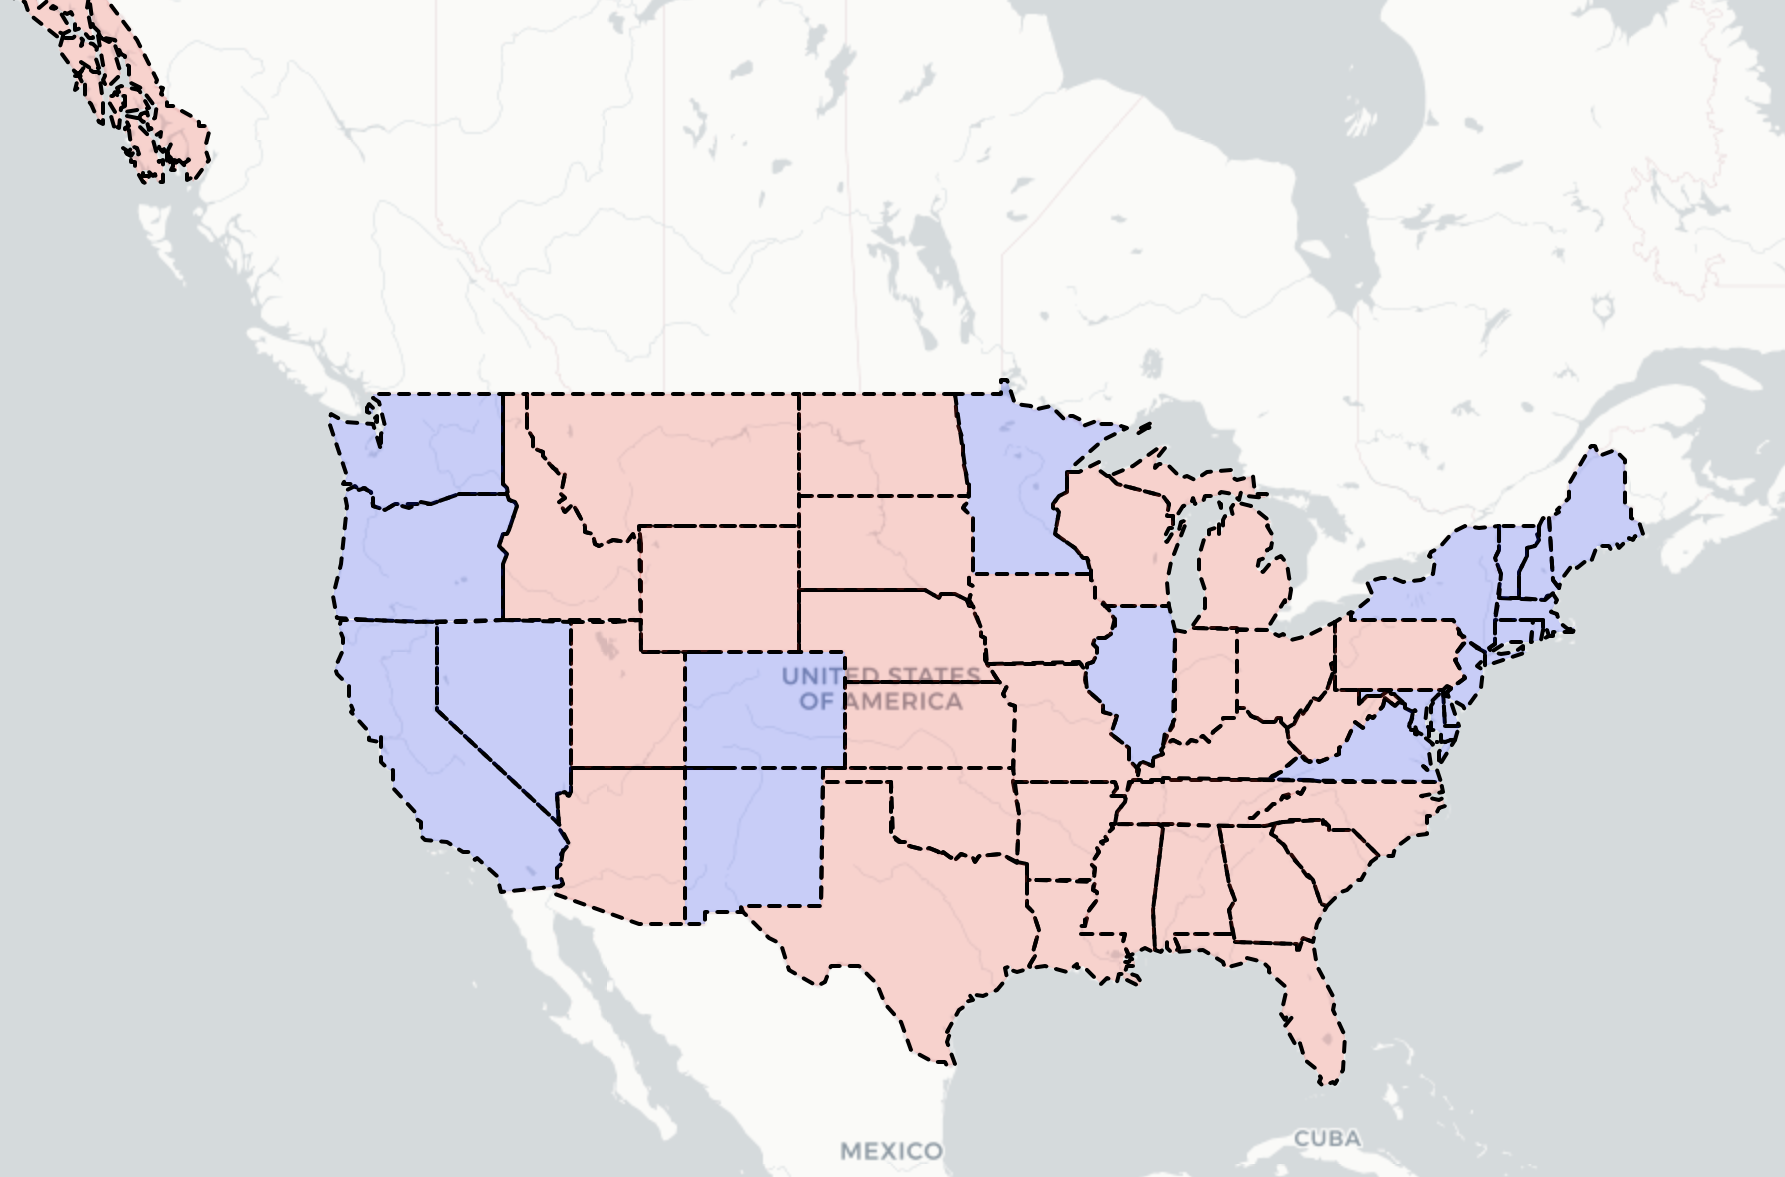
\includegraphics[scale=0.15]{Images/real_results.png}
\caption{Actual results : Blue means that Clinton won, Red means Trump won.}
\label{US_result}
\end{figure}

\begin{figure}[!h]
\centering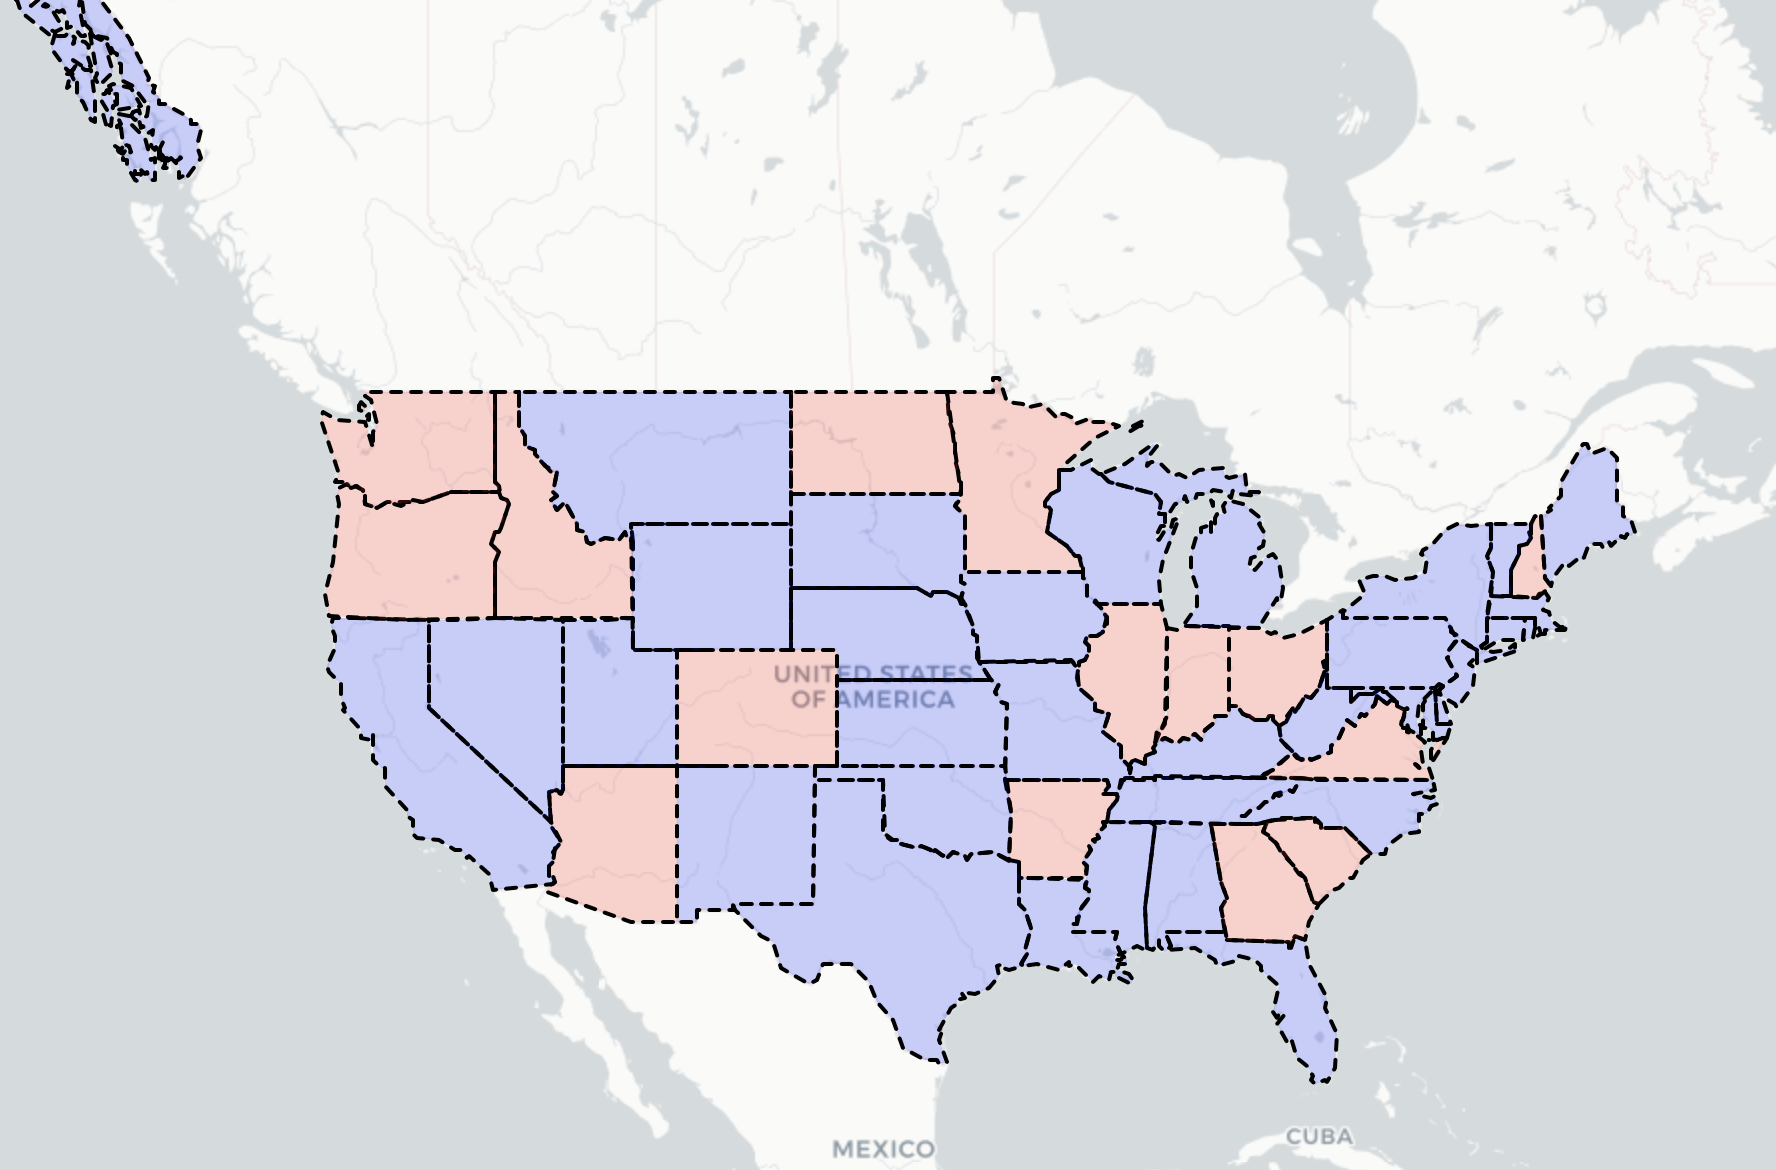
\includegraphics[scale=0.15]{Images/disregarding_scores.png}
\caption{Predicted results disregarding the score: The accuracy is 21 out of 50}
\label{US_prediction}
\end{figure}

\begin{figure}[!h]
\centering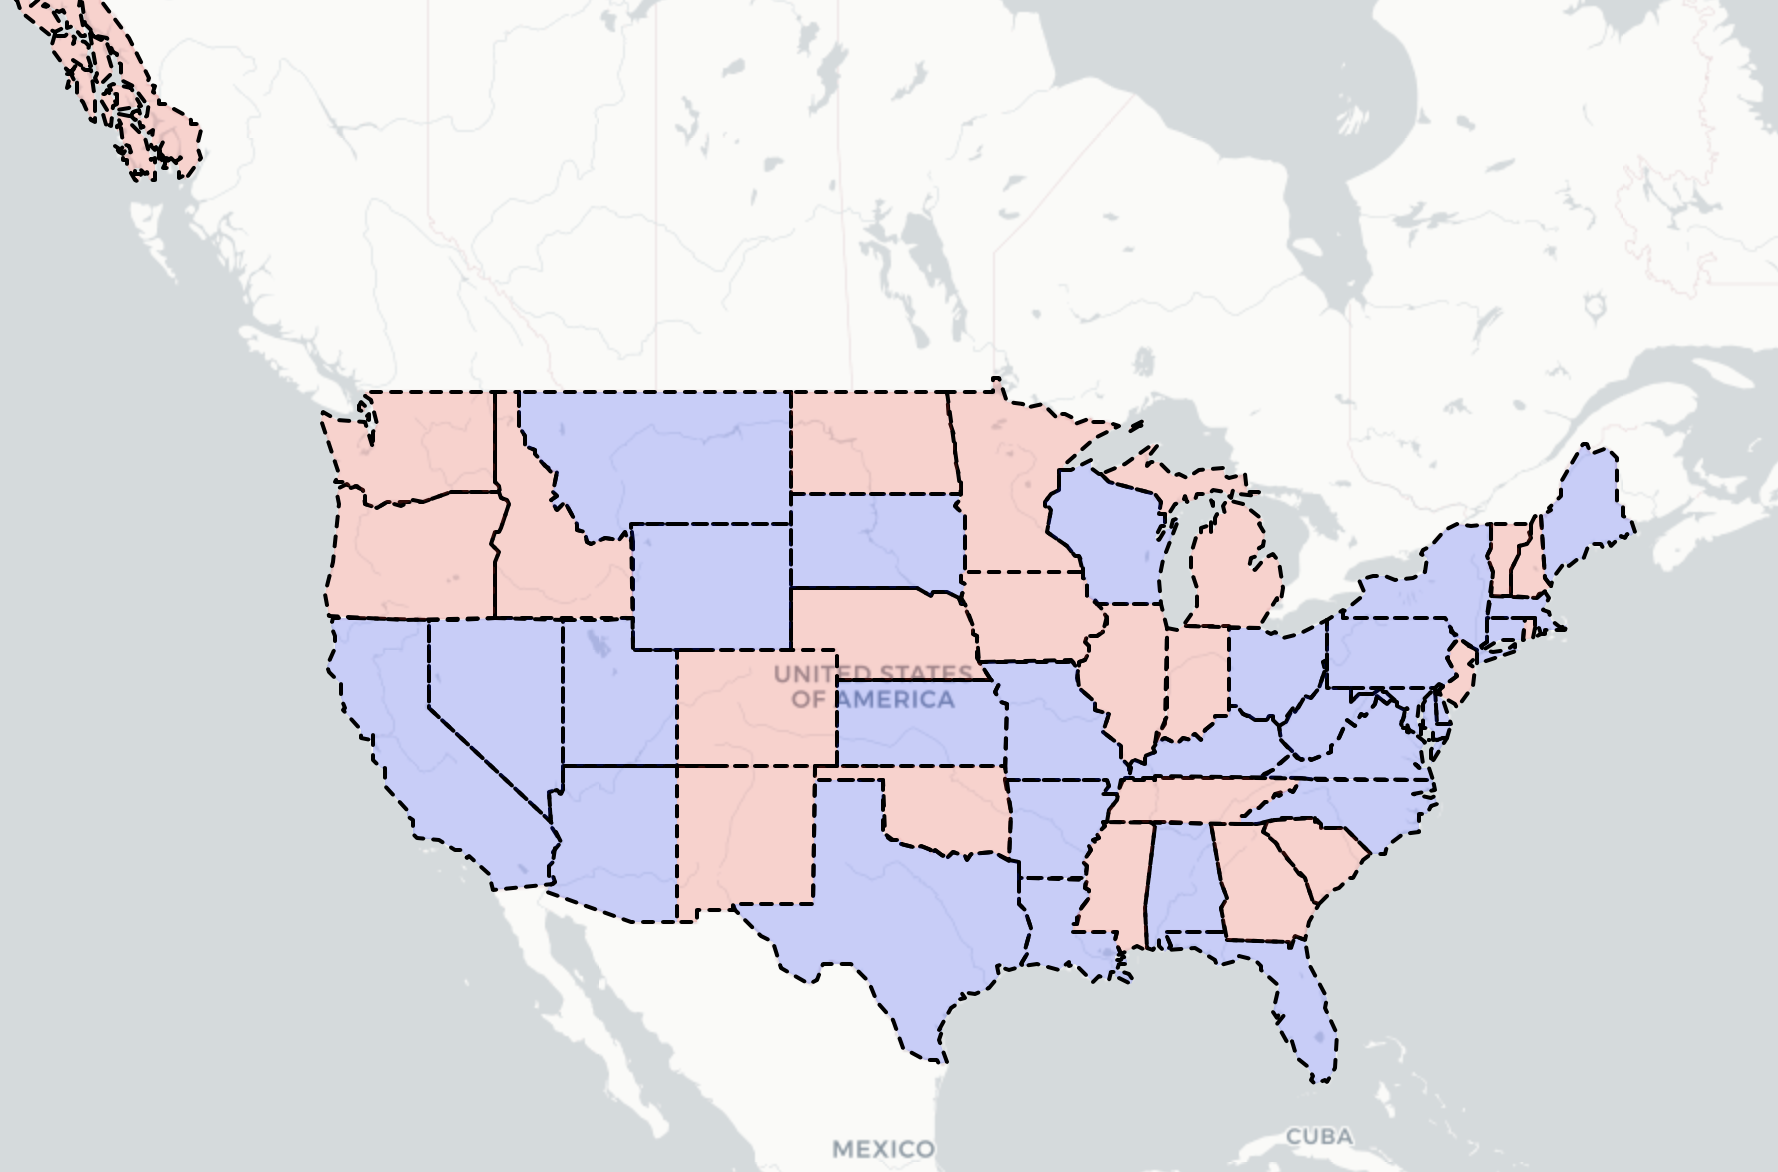
\includegraphics[scale=0.15]{Images/weighted_scores.png}
\caption{Prediction using a weighted score : The accuracy is 22 out of 50}
\label{US_prediction_weighted}
\end{figure}

From the data collected, the best prediction made was found in Figure \ref{US_prediction_weighted}, where 22 out of the 50 states were correct. This was computed using a 0.2 weighted score. 
The difference between our predictions and real election results is important, but this can be explained by many things, but mainly by the fact that we considered the data set with the flair feature corresponding to a US state, since otherwise we cannot guarantee the origin of our users and hence a score for a state cannot be made. Also, some states like South Dakota or Delaware were not well represented.
\subsection{Scores}
For every category, the 10 best words are almost always the same, with some order difference. The 10 best words in these category are \textit{"Trump"} (10483 mentions max) ,\textit{"like", "people", "Clinton", "would", "Hillary", "one", "get", "vote"} and \textit{"party"} (2378 mentions).\\
Since all the words are both good and bad, it is not a good indicator. The good and bad words that appear only on their side can be seen in the following lists.

\begin{description}
    \item[Good words only] \textit{"whois"} (76 mentions) ,\textit{"Indianapolis", "oylyhig", "Fahrenthold", "FDNY", "RFRA"} and \textit{"downgrade"} (29).
\end{description}

\begin{description}
    \item[Bad words only] \textit{"iujghuikzy\footnote{https://www.youtube.com/watch?v=5IuJGHuIkzY}"} (72 mentions) ,\textit{"Kerrey", "hdc", "precautionary", "pimped", "vol"} and \textit{"stoning"} (16).
\end{description}

As it can be seen from the previous lists, there is no strong good or bad word, since most of the words appears in both sets.  
 
\subsection{Popularity Evolution}
The compound analysis gave us the evolution of the sentiment after certain political events. For example, we can see that when Obama publicly endorses Hillary (June \nth{9}), more positive comments were posted concerning Hillary than Trump. Another one is when the FBI scandal concerning Hillary Clinton was announced, her popularity drastically dropped. For more details, see Figure \ref{Popularity_score}.

\begin{figure*}[!h]
\centering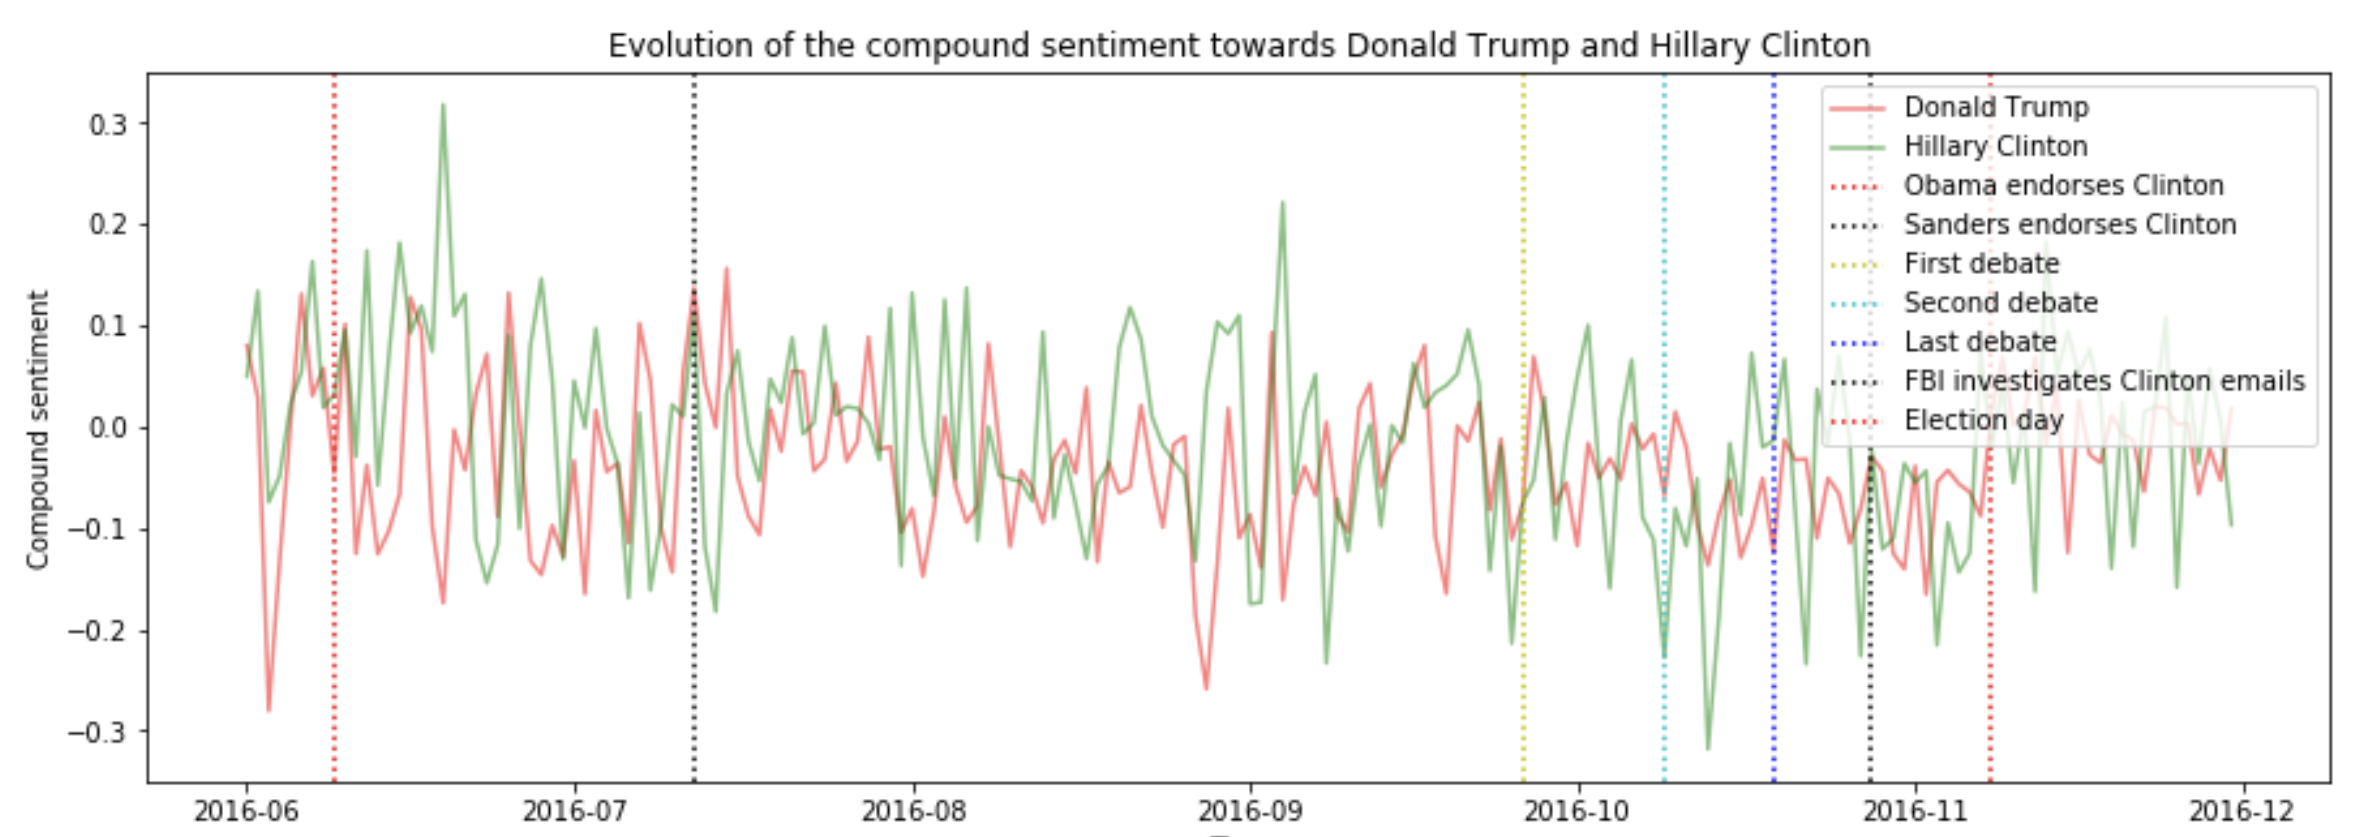
\includegraphics[width=\textwidth]{Images/compound_ev.png}
\caption{Compound Polarity Score}
\label{Popularity_score}
\end{figure*}

The positive and negative comments distribution completed our sentiment evolution analysis concerning the candidates. We can see in Figure \ref{Trump_hist} that Trump is mentioned a lot more than Hillary, but that is not necessarily a good sign since the majority of the comments are labeled as negative. However, Hillary was overall mentioned positively right until the second debate period and the FBI investigation scandal. The number of  comments mentioning Trump positively and negatively is shown in Figure \ref{Trump_hist}.

\begin{figure}[H]
\centering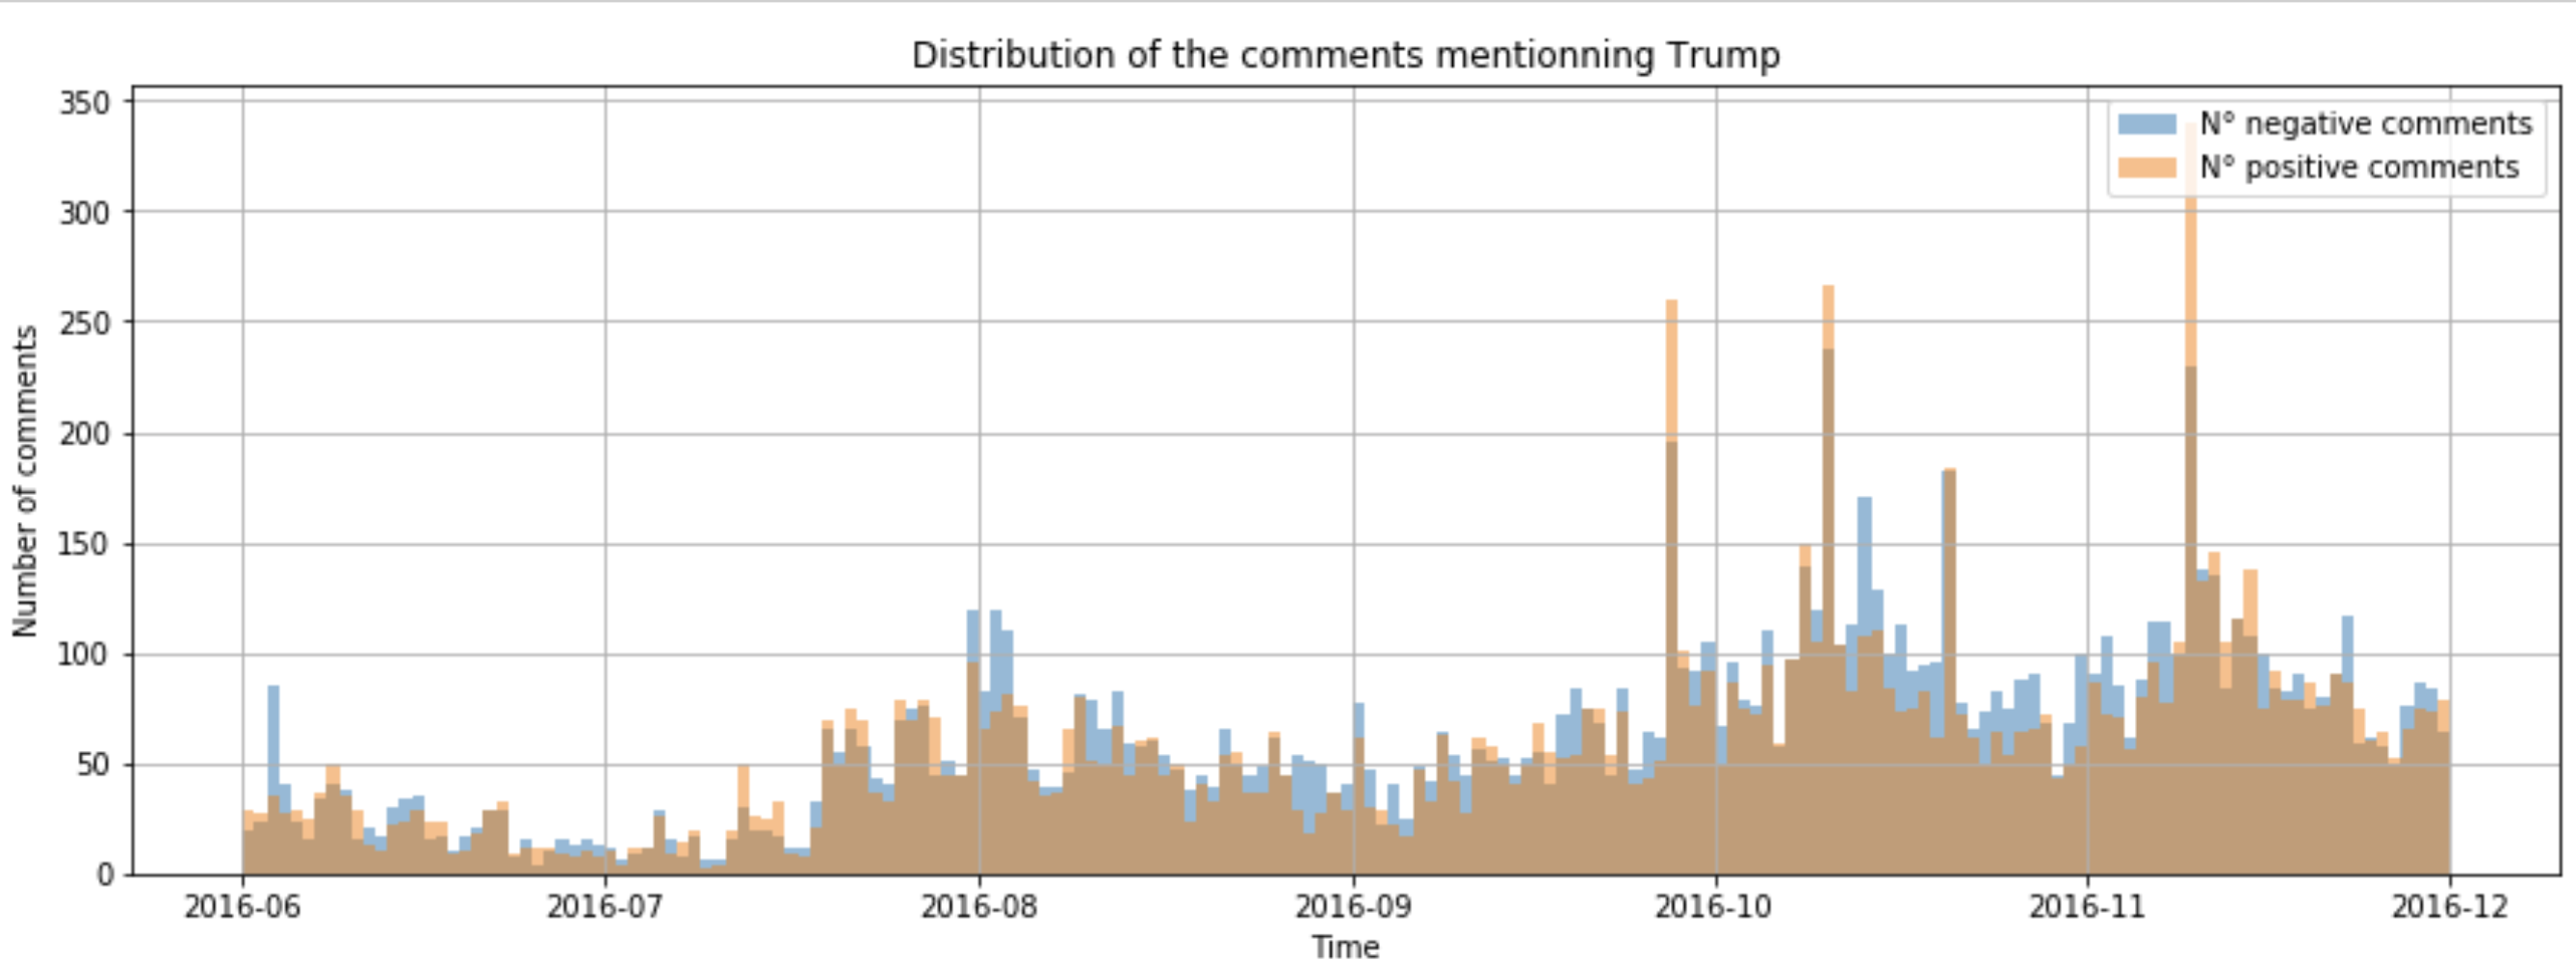
\includegraphics[scale=0.17]{Images/trump_comments.png}
\caption{Number of positive and negative comments mentioning Trump}
\label{Trump_hist}
\end{figure}


\section{Conclusion}
In this project, we discovered the underlying patterns that can contribute into making a Reddit comment deemed good by other users (words such as "RFRA" which means Religious Freedom Restoration Act, is a US law). We also analyzed the comments' polarity according to actual political events, and we saw that if a scandal regarding a particular candidate breaks out for example, its popularity downgrades. In addition, we tried to predict, using these comments, the outcome of the 2016 American presidential election. We can see that the results of the predictions differ a lot with the actual ones, and this was not surprising. Indeed, the Reddit users are not constituted by the entire US population, some users do not even have the legal age to vote, and we only used the comments that had their author flair set to a US state. Moreover, more data concerning certain states would have been more insightful. We can hence conclude by saying that predicting the outcome of an election using only one social media platform and a data set of 215'000 comments will not lead to necessarily true results.

\end{document}
